We now want to address the numerical solution of fluid-structure interaction problems.
In order to address each problem in its natural setting, we
choose to consider the fluid in an ALE (Arbitrary Lagrangian
Eulerian) formulation and the structure in a pure Lagrangian framework.


\ixn{Fluid-Structure Interactions}

The system under investigation occupies a moving domain $\Omegat$
in its actual configuration. It is made of a deformable structure
$\OmegaSt$ (such as an arterial wall, a pipe-line, \ldots)
surrounding a fluid under motion (blood, oil, \ldots) in  the
complement $\OmegaFt$ of  $\OmegaSt$ in $\Omegat$ (see
Fig.~\ref{fig:ALEmapping}).

\begin{figure}[!h]
\begin{center}
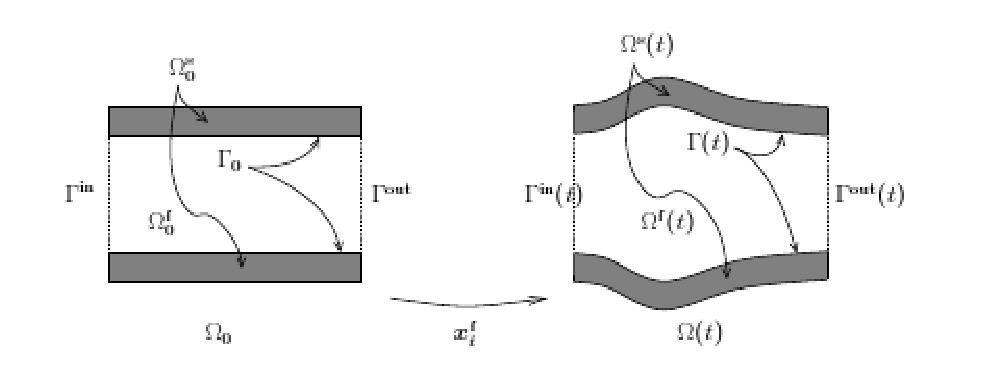
\includegraphics[width=.8\textwidth]{ALEmapping.pdf}
\end{center}
\caption{ALE mapping between the initial configuration and the
configuration at time $t$.}\label{fig:ALEmapping}
\end{figure}

We assume the fluid to be Newtonian, viscous, homogeneous and
incompressible. Its behavior is described by its velocity and
pressure. The elastic solid under large displacements is
described by its velocity and its stress tensor. The classical
conservation laws of the continuum mechanics govern the evolution
of these unknowns.

We denote by $\GamInt$ and $\GamOut$ the inflow and outflow
sections of the fluid domain, by $\uu n_\mf$ the  fluid domain's
outward normal on $\partial \OmegaFt$ and by $\uu n_\ms$ the one
of the structure on the reference boundary $\partial \hOmegaS$.
The boundary conditions on the fluid inlet and outlet can be
either natural or essential (i.e., of Neumann or Dirichlet type,
respectively), while on the interface we impose that the fluid
and structure velocities match and so do the normal stresses. For
simplicity, we assume zero body forces on both the structure and
the fluid and that the boundary conditions on the remaining part
of the structure boundary are of Dirichlet or of Neumann type.

The problem consists in finding the time evolution of the
configuration $\OmegaFt$, as well as the velocity $\uu u$ and
pressure $p$ for the fluid and the displacement $\D$ of
the structure. We define the ALE mapping
\begin{equation*}
 \forall t \,,\;  \ALE{t} : \hOmegaF \rightarrow \OmegaFt,
\end{equation*}
i.e. a map that retrieves at each time the current configuration
of the computational domain $\OmegaFt$. Note in particular that on
the reference interface $\hWall$, $\uu n_\mf \circ \ALE{t} = -\uu
n_\ms$. We denote by $\bY$ the coordinates on the reference
configuration $\hOmegaF$ and by $\bw=\frac{d \ALE{t}}{dt}$ the
domain velocity.

%%%%%%%%%%%%%%%%%%%%%%%%%%%%%%%%%%%%%%%%%%%%%%%%%%%%%%%%%%%%%%%%%%%%%%
\medskip
For simplicity, we denote in short by $\NS(\ldots)$ and
$\Str(\ldots)$ the fluid and structure problems, respectively.
Precisely, for given vector functions $\uu u_\In$, $\uu g_\mf$ and
$\uu f_\mf$, $\NS(\U,p,\ALE{t};\uu u_\In, \uu g_\mf, \uu f_\mf)$
means that we consider the following problem whose solution is
$\U$, $p$ and $\ALE{t}$:
\begin{equation}\label{eq:fluid}
  \NS(\U,p,\ALE{t};\uu u_\In, \uu g_\mf, \uu f_\mf):
  \begin{cases}
    \dis  \uu \Delta \ALE{t} = 0 \text{ in } \hOmegaF, \\
    \dis  \ALE{t} = 0 \text{ on } \partial\hOmegaF \setminus\hat\Sigma, \\
    \dis  \OmegaF_{t} = \ALE{t}(\hOmegaF), \\
    \dis  \rho_\mf\left(\diffALE \U + (\U-\bw)\cdot \Grad \U\right) \\
    \dis  \qquad = \Div (2\mu\uu \epsilon(\U)) - \Grad p  + \uu f_\mf \text{ in }\OmegaF_{t}, \\
    \dis  \Div\U=0 \text{ in }\OmegaF_{t},\\
    \dis  \U = \uu u_\In \text{ on } \GamIn_t,\\
    \dis  \uu\sigma_\mf (\uu u,p)\cdot\uu n_\mf = \uu g_\mf \text{ on }\GamOu_{t},
  \end{cases}
\end{equation}
where $\rho_\mf$ is the fluid density, $\mu$ its viscosity,
$\strain(\U) = \Strain u$ is the strain rate tensor and $\uu
\sigma_\mf(\U,p)=-p Id + 2\mu\strain(\U)$ the Cauchy stress
tensor ($ Id $ is the identity matrix). Note
that~(\ref{eq:fluid}) does not univocally define a solution
$(\U,p,\ALE{t})$ as no boundary data are prescribed on the
interface $\Sigma_t$.

Similarly, for given vector functions $\uu g_\ms$, $\uu f_\ms$, $\Str(\D;\uu g_\ms, \uu f_\ms)$ means that
we consider the following problem whose solution is $\D$:
\begin{equation}\label{eq:struct}
  \Str(\D;\uu g_\ms, \uu f_\ms) :
  \begin{cases}
    \dis  \rho_\ms \frac{\partial^2 \D}{\partial t^2} = \Div(\uu \sigma_\ms(\D))
    -\gamma \D +\uu f_\ms \text{ in }\hOmegaS, \\
    \dis  \uu\sigma_\ms(\D) \cdot {\uu n}_\ms = \uu g_\ms
    \text{ on }\partial\hOmegaS\setminus\hGamW,
  \end{cases}
\end{equation}
where $\piola(\D)$ is the first Piola--Kirchoff stress tensor,
$\gamma$ is a coefficient accounting for possible viscoelastic
effects, while $\uu g_\ms$ represents the normal traction on
external boundaries. Appropriate models have to be chosen for the
structure depending on the specific problem at hand.

Similarly to what we have noticed for~(\ref{eq:fluid}),
problem~(\ref{eq:struct}) can not define univocally the unknown
$\D$ because a boundary value on $\hGamW$ is missing.

When coupling the two problems together, the ``missing'' boundary
conditions are indeed supplemented by suitable matching
conditions on the reference interface $\hWall$. More precisely,
if we denote by $\lambda$ the interface variable corresponding to
the displacement $\D$ on $\hWall$, at any time the coupling
conditions on the reference interface $\hWall$ are
\begin{equation}\label{eq:condizioni}
\begin{array}{c}
  \ALE{t} = \lambda ,\\[4pt]
  \U \circ \ALE{t} = \dot{\D}_{\hWall} ,\\[4pt]
  (\uu \sigma_\mf(\U,p) \cdot {\uu n}_\mf) \circ \ALE{t} +
  \uu \sigma_\ms(\D)\cdot {\uu n}_\ms =0,
\end{array}
\end{equation}
where $\dot{\D}_{\hWall}$ denotes the temporal derivative of
$\D_{\vert\hWall}$. The system of equations (\ref{eq:fluid})-(\ref{eq:condizioni})
identifies our coupled fluid-structure problem.
We suppose the problem to be discretized in time. When the
solution is available at time $t^n$, we look for the solution at
the new time level $t^{n+1} = t^n + \delta t$. If no ambiguity
occurs,  all the quantities will be referred to at time
$t=t^{n+1}$.
Without loss of generality we consider zero body forces, i.e.,
$\uu f_\mf =0$ and $\uu f_\ms=0$.

If we are given a displacement of the interface  $\lambda(t^{n+1})$ at the
time $t^{n+1}$, we can find its harmonic extension on the fluid domain by solving
the  following variational formulation of
(\ref{eq:harmonicextension}):

find $\Df_{t^{n+1}} \in H^1(\DomFi)^3$ such that
\begin{equation} \label{eq:variationalvelocity2}
\left\{
\begin{array}{rcl}
\dis \int_{\DomFi} \Grad \Df_{t^{n+1}}\cdot \Grad \uu \phi  =  0 & & \forall \uu \phi \in H^1_0(\DomFi)^3\\
\Df_{t^{n+1}} = \lambda({t^{n+1}}) & & \text{on } \GamFSi,
\end{array}
\right.
\end{equation}
completed with appropriate boundary conditions  on $\GamIn\cup\GamOu$.

Then we compute the velocity of the fluid domain as 
$\dis \wf{}^{,n+1}_{|\GamFS{n+1}} = 1/\delta t\,(\Df_{t^{n+1}}{}_{|\GamFSi} - \Df_{t^n}{}_{|\GamFSi})
\circ(\ALE {t^{n+1}})^{-1}$ and the velocity and pressure of the fluid at time
$t^{n+1}$ by solving:

find $(\U^{n+1},p^{n+1}) = (\U(t^{n+1}),p(t^{n+1})) \in V^\mf(t^{n+1})\times Q^\mf(t^{n+1})$ such
that $\U^{n+1}_{|\GamFS{n+1}} =  \wf{}^{,n+1}_{|\GamFS{n+1}}$,
$\U^{n+1}_{|\GamIn(t^{n+1})} =  \U_\In(t^{n+1})$
and
\begin{equation} \label{eq:variationalfluid}
\left\{
\begin{array}{l}
\displaystyle \frac{1}{\delta t}\int_{\DomF(t^{n+1})} \rho_\mf \U^{n+1}\V^\mf
+ \displaystyle \int_{\DomF(t^{n+1})}\rho_\mf [(\U^{n+1} -  \wf{}^{,n+1})\cdot \Grad \U^{n+1}]\V^\mf\\ \quad
\displaystyle + \mu\int_{\DomF(t^{n+1})} \Fstress[{n+1}] \cdot \Grad \V^{\mf}
= \displaystyle \frac{1}{\delta t} \int_{\DomF(t^{n+1})} \rho_\mf \U^n \V^\mf +
\int_{\Gamma^{\mathrm{out}}(t^{n+1})} \uu g_{\mf} \V^\mf \\
\displaystyle \int_{\DomF(t^{n+1})} q^\mf \Div \U^{n+1}  = 0
\end{array}
\right.
\end{equation}
for all $(\V^\mf,q^\mf) \in V_0^\mf(t^{n+1}) \times Q^\mf(t^{n+1})$, with
\begin{eqnarray*}
V^\mf(t) & = & \left\{\V^\mf \vert \,   \V^\mf \circ \ALE {t}  \in H^1(\DomFi)^3\right\}, \\
V_0^\mf(t) & = & \left\{\V^\mf \in V^\mf(t) \vert \,\V^\mf  \circ \ALE {t}
= \mathbf{0} \mbox { on } \GamFSi \cup \GamIn \right\}, \\
Q^\mf (t)& = & \left\{q^\mf  \vert \, q^\mf \circ \ALE {t} \in L^2(\DomFi)\right\},
\end{eqnarray*}
and where the fluid domain $\DomF(t^{n+1})$ is given by
\begin{equation*}
\DomF(t^{n+1})  = \ALE {t^{n+1}}(\DomFi).
\end{equation*}

We can then compute $  (\Fstress[{n+1}] \cdot {\uu n}_\mf) \circ \ALE t $ on $ \GamFSi$,
which by (\ref{eq:couplingconditions}) has to be equal to the structure normal stresses.
%We call $\Sf$ the operator that given $\lambda$ computes $S_\mf(\lambda)= \sigma_\mf$.


On the structure side, given the same displacement $\lambda(t^{n+1})$, we can use the
following scheme to approximate the arterial deformation and the domain
velocity (see \cite{FerMou04:NewtonFS}):

find $(\ds{}^{,n+1},\ws{}^{,n+1})=(\ds(t^{n+1}),\ws(t^{n+1})) \in V^\ms\times
V^\ms$ such that
\begin{equation} \label{eq:variationalstructure}
\left\{
\begin{array}{rl}
%    \dis  \int_{\DomSi} \rho_\ms \frac{\partial^2 \uu d^\ms}{\partial t^2}v^\ms
    \dis  \frac{2}{\delta t^2} \int_{\DomSi} \rho_\ms \ds{}^{, n+1} \V^\ms
    &\dis-  \frac{2}{\delta t^2} \int_{\DomSi} \rho_\ms (\ds{}^{, n} + \delta t \ws{}^{, n})\V^\ms
    +  \int_{\DomSi} \Sstress(\ds{}^{, n+1})\cdot \Grad \V^\ms    \\
    &\dis = \int_{\partial\DomSi\setminus\GamFSi} \uu g_\ms \cdot \V^\ms\\
    \dis \uu w^{\ms,n+1} &\dis=  \frac{2}{\delta t}(\uu d^{\ms,n+1} - \uu d^{\ms,n}) - \ws{}^{,n}\\
    \dis\uu d^{\ms,n+1} &\dis =  \lambda(t^{n+1}) \quad\text{ on } \GamFSi,
    \end{array}
\right.
\end{equation}
for all $\V^\ms \in V^\ms$ such that $\V^\ms_{|\GamFSi} = 0$,
with $V^\ms = H^1(\DomSi)^3 $. As for the fluid, we can then compute the structure
normal stresses on the interface  as $\Sstress(\Ds{}^{, n+1}) \cdot {\uu n}_\ms$  on $\GamFSi$.

If for a given interface displacement $\lambda(t^{n+1})$ the fluid and structure normal stresses are
at equilibrium,
%  i.e.,
% $(\Fstress \cdot {\uu n}_\mf) \circ \ALE t +
% \Sstress(\Ds) \cdot {\uu n}_\ms = 0$,
%$ \sigma_\mf + \sigma_\ms = 0$,
it means that the fluid-structure problem has
been correctly solved.
In general we impose the equilibrium in weak form, i.e.,
\begin{multline*}
  \int_{\GamFS{n+1}} \Fstress \cdot \uu n_{\mf}\V^\mf + \int_{\GamFSi}
  \Sstress(\Ds) \cdot \uu n_{\ms} \V^s = 0 \\
  \forall (\V^\mf,
  \V^\ms) \in V^\mf(t^{n+1}) \times V^\ms \text{ s.t. } \V^\mf\circ\ALE t =
  \V^\ms \text{ on } \GamFSi.
\end{multline*}
Both integrals can be computed as residuals of
the weak form of the equations.
We consider the coupled problem at a particular time  $t=t^{n+1}$.
In order to write the interface equation associated to the global
fluid-structure problem, we introduce a fluid and structure operator
as follows.

Let $\Sf$ be the Dirichlet-to-Neumann (D-t-N) fluid map such that to any given interface
displacement $\lambda$ it associates the normal stress
$$
\Sf (\lambda) = \sigma_\mf :=  (\Fstress \cdot {\uu n}_\mf) \circ \ALE t \mbox{ on } \GamFSi,
$$
where $(\U, p)$ is the solution of the Navier-Stokes problem (\ref{eq:variationalfluid}). On the
other hand, we denote by $\Ss$ the D-t-N operator associated to the structure in $\GamFSi$ such
that to any given displacement $\lambda$ of the interface $\GamFSi$ it associates the normal stress
exerted by the structure on $\GamFSi$:
$$
\Ss (\lambda) = \sigma_\ms :=  (\Sstress(\Ds) \cdot {\uu n}_\ms) \mbox{ on } \GamFSi,
$$
where $\Ds$ is the solution of (\ref{eq:variationalstructure}).

Concerning the inverse of the solid operator, we can define $S_\ms^{-1}$ as a Neumann-to-Dirichlet
(N-t-D) map that at any given normal stress $\sigma$ on $\GamFSi$ associates the interface
displacement $\lambda(t^{n+1}) = \D^{\ms,n+1}$ by solving a structure problem analogous to
(\ref{eq:variationalstructure}), but with the Neumann boundary condition
\begin{equation*}
\uu \sigma_\ms(\D^s) \cdot\uu n_\ms = \sigma \textrm{ on } \GamFSi
\end{equation*}
and then computing the restriction on $\GamFSi$ of the displacement of
the structure domain.

Moreover, we denote by $S_\ms'$ the tangent operator associated to the structure problem and by
$(S_\ms')^{-1}$ its inverse. The latter is a N-t-D map that to any given normal stress $\sigma$ on
$\GamFSi$ associates the corresponding displacement $\lambda(t^{n+1})$ of the interface by solving
the linearized structure problem with boundary condition $\boldsymbol{\sigma}_\ms (\Ds) \cdot \uu
n_\ms = \sigma$ on $\GamFSi$. Analogously, by $(S_\mf')^{-1}$ we denote the inverse of the tangent
operator $S_\mf'$. This is also a N-t-D map  that for any given normal stress $\sigma$ on $\GamFSi$
computes the corresponding displacement $\lambda(t^{n+1})$ of the interface through the solution of
linearized Navier-Stokes equations with the boundary condition $(\Fstress \cdot {\uu n}_\mf) \circ
\uu x^{\mf} = \sigma$ on $\Gamma_0$.
Using the definitions of the operators $\Sf$ and $\Ss$ and of their inverses, we can express the
coupled fluid-structure problem in terms of the solution $\lambda$ of a nonlinear equation defined
only on $\GamFSi$. More precisely, we can envisage three possible formulations for the interface
equation which are all equivalent from a mathematical point of view, but give rise to different
iterative methods.

First, we have the fixed-point formulation
\begin{equation} \label{eq:fixedpoint}
\mbox{find } \lambda \mbox { such that } \Ss^{-1}(-\Sf(\lambda)) = \lambda
\mbox{ on } \GamFSi .
\end{equation}
This is a classical formulation in fluid-structure interaction problems, but it is worth pointing
out that here the fixed point is the displacement of the sole interface, whereas in the
literature the solution obtained via
fixed-point algorithms usually represents the displacement of the whole solid domain.

The second possible approach is a slight modification of the previous equation
(\ref{eq:fixedpoint})
\begin{equation} \label{eq:newton}
\mbox{find } \lambda \mbox { such that } \Ss^{-1}(-\Sf(\lambda)) - \lambda = 0 \mbox{ on } \GamFSi,
\end{equation}
which is more suitable for setting up a Newton iterative method.
Again, this is applied solely to the interface displacement,
instead of the whole solid displacement as proposed.

Let's have a look at the code located at \verb!testsuite/test_fsi/main.cpp!. The first interesting part
is the problem definition part, starting from these lines 
\begin{verbatim}
    Problem( GetPot const& data_file, std::string _oper = "" )
        {
            using namespace LifeV;

            debugStream( 10000 ) << "creating FSISolver with operator :  " << _oper << "\n";

            M_fsi = fsi_solver_ptr(  new FSISolver( data_file, _oper ) );
            debugStream( 10000 ) << _oper << " set \n";

            MPI_Barrier(MPI_COMM_WORLD);
\end{verbatim}

This will create a new fluid/structure interaction problem that will be solved using a
non-linear Richardson algorithm on the following interface equation 

\begin{equation}\label{eqn-interface}
\lambda^{k+1}  =  \lambda^k + \omega^k f(\lambda^k),
\end{equation}
where $f$ depends on the chosen FSI method. If we look at the FSI problem constructor
the file \verb!life/lifesolver/FSISolver.cpp!, we have 

\begin{verbatim}
FSISolver::FSISolver( GetPot const& data_file,
                      std::string   __oper ):
    M_lambda      (),
    M_lambdaDot      (),
    M_firstIter (true),
    M_method    ( data_file("problem/method"     , "steklovPoincare") ),
    M_maxpf     ( data_file("problem/maxSubIter" , 300) ),
    M_defomega  ( data_file("problem/defOmega"   , 0.01) ),
    M_abstol    ( data_file("problem/abstol"     , 1.e-07) ),
    M_reltol    ( data_file("problem/reltol"     , 1.e-04) ),
    M_etamax    ( data_file("problem/etamax"     , 1.e-03) ),
    M_linesearch( data_file("problem/linesearch" , 0) ),
    M_epetraComm(),
    M_epetraWorldComm(),
    M_localComm (new MPI_Comm),
    M_interComm (new MPI_Comm),
    out_iter    ("iter"),
    out_res     ("res")
\end{verbatim}


where
\begin{itemize}
\item \verb!M_lambda! is the interface displacement as defined in (\ref{eq:condizioni}),
\item \verb!M_lambdaDot! is the temporal derivative of \verb!M_lambda!.
\end{itemize}
See table \ref{table-fsiparams} for a complete of these options of options.

\begin{table}[!h]
\begin{center}
\begin{tabular}{|l|l|l|}
\hline
Name & Options & Description \\
\hline \hline
method & fixedPoint & FSI resolution method name\\
& exactJacobian & \\
\hline
maxSubIter & 300 & maximum nonlinear Richardson iterations \\
\hline
defOmega & 0.01 & default step in (\ref{eqn-interface}) (deprecated) \\
\hline
abstol & 1e-07 & abstol and reltol define the stoping \\
reltol & 1e-04 & criteria as abstol+reltol*norm(residual0) \\
& & where residual0 is the first nonlinear Richardson \\
& & FSI evaluation residual. \\
\hline
etamax & 1e-03 &  Maximum error tolerance for residual in the linear solver. \\
\hline
linesearch & 0 & nonlinear Richardson algorithm linesearch \\
& & (always use 0, i.e no line search, for now).\\
monolithic & 0 & monolithic description of the FSI problem \\
& & (under development)\\
\hline

\end{tabular}
\end{center}
\caption{ FSI problem data file parameters
%\ixt{FSI data parameters}{data parameters}
}
\label{table-fsiparams}
\end{table}


The \verb!monolithic! description of the FSI problem is still under  development and
should not be used for now. Let's have the look at the rest of the FSI problem constructor code.

\begin{verbatim}
 MPI_Group  originGroup, newGroup;
 MPI_Comm   newComm;

 MPI_Comm_group(MPI_COMM_WORLD, &originGroup);

 if (numtasks == 1)
     {
         std::cout << "Serial Fluid/Structure computation" << std::endl;
         newComm = MPI_COMM_WORLD;
         fluid = true;
         solid = true;
         fluidLeader = 0;
         solidLeader = 0;

         M_epetraWorldComm.reset(new Epetra_MpiComm(MPI_COMM_WORLD));
         M_epetraComm = M_epetraWorldComm;

     }
 else
     {
         int members[numtasks];

         solidLeader = 0;
         fluidLeader = 1 - solidLeader;

         if (rank == solidLeader)
             {
                 members[0] = solidLeader;
                 int ierr;
                 ierr = MPI_Group_incl(originGroup, 1, members, &newGroup);
                 solid = true;
             }
         else
             {
                 for (int ii = 0; ii <= numtasks; ++ii)
                     {
                         if ( ii < solidLeader)
                             members[ii] = ii;
                         else if ( ii > solidLeader)
                             members[ii - 1] = ii;
                     }
                 int ierr;
                 ierr = MPI_Group_incl(originGroup,
                                       numtasks - 1,
                                       members,
                                       &newGroup);
                 fluid = true;
             }

         MPI_Comm* localComm = new MPI_Comm;
         MPI_Comm_create(MPI_COMM_WORLD, newGroup, localComm);
         M_localComm.reset(localComm);

         M_epetraComm.reset(new Epetra_MpiComm(*M_localComm.get()));
         M_epetraWorldComm.reset(new Epetra_MpiComm(MPI_COMM_WORLD));
     }

\end{verbatim}

This part is dedicated at assigning jobs to the different processors. Since we have to deal
with a separate structure and fluid problems, we define two MPI groups where for each problem.
For now, by convention, and since the structure problem is resolved more easily than the
fluid problem by far, the structure group has only the \#0 (leader) processor, whereas the fluid group is
composed of all the other processors. At the end of these lines, two MPI intracommunicators
(communicator within a single group of processes), one for the structure,
one for the fuid, and one MPI intercommunicator (communicator within two or
more groups of processes) are created. See \url{http://www.mpi-forum.org/docs/mpi-11-html/mpi-report.html}
for more information on intra and intercommunicators.

From now on, each processor knows if it belongs to the structure or the fluid group. This is
very important since each group will create its own problem, either stucture of fluid.
Since the structure problem requires less ressources than the fluid problem, the FSI problem defined in (\ref{eqn-interface})
will be solved on a lead structure processor (\#0 processor within the structure intracommunicator).

\begin{verbatim}


    Preconditioner precond  = ( Preconditioner )
                               data_file("problem/precond"   ,
                               DIRICHLET_NEUMANN );

    debugStream( 6220 ) << "FSISolver::preconditioner: " << precond << "\n";

    if ( !__oper.empty() )
    {
        M_method = __oper;
    }

    debugStream( 6220 ) << "FSISolver::setFSIOperator " << M_method << "\n";

    this->setFSIOperator( M_method );

    M_oper->setFluid(fluid);
    M_oper->setSolid(solid);

    M_oper->setFluidLeader(fluidLeader);
    M_oper->setSolidLeader(solidLeader);

    debugStream( 6220 ) << "FSISolver::setPreconditioner " << precond << "\n";

    std::cout << std::flush;
    M_oper->setComm(M_epetraComm, M_epetraWorldComm);

    debugStream( 6220 ) << "FSISolver::setDataFromGetPot " << precond << "\n";
    std::cout << std::flush;

    M_oper->setDataFromGetPot( data_file );


    debugStream( 6220 ) << "FSISolver::setPrecond " << precond << "\n";
    std::cout << std::flush;

    M_oper->setPreconditioner( precond );

    M_oper->setup();

    debugStream( 6220 ) << "FSISolver:: variable setup " << precond << "\n";

    M_oper->setUpSystem(data_file);

    M_lambda.reset   (new vector_type(*M_oper->solidInterfaceMap()));
    M_lambdaDot.reset(new vector_type(*M_oper->solidInterfaceMap()));
    M_oper->buildSystem();

\end{verbatim}

This part  creates the proper numerical FSI Operator (fixed point, exact jacobian, ...)
for solving (\ref{eqn-interface}), that is the fluid and the structure operators ($S_f$, $S_s$ ... )
defined previously, and set them up. You can have a look at the code which is in \verb!life/lifesolver/FSIOpertator.hpp,cpp!,
\verb!life/lifesolver/exactJacobianBase.hpp,cpp! and \verb!life/lifesolver/fixedPointBase.hpp,cpp!.
The last two classes, exactJacobian and fixedPoint, derive from the class FSIOperator, which only
deals with passing information (displacement or constrain) from the solid or the fluid to the fluid or solid via
the interface. The the specialized classes exactJacobian or fixedPoint evalute the interface residual
and solve $f(\lambda)$ as defined in (\ref{eqn-interface}).
The last interesting part in the \verb!FSISolver! class, is the \verb!iterate! member
\begin{verbatim}
    M_oper->setTime(time);

    fct_type fluidSource(zero_scalar);
    fct_type solidSource(zero_scalar);

    if(!M_monolithic)
        M_oper->updateSystem(fluidSource, solidSource);
    else
        M_oper->updateSystem(*M_lambda);

    // displacement prediction
    MPI_Barrier(MPI_COMM_WORLD);

    if (M_firstIter)
    {
        M_firstIter = false;

        if(!M_monolithic)
            {
                *M_lambda      = M_oper->lambdaSolid();
                *M_lambda     += timeStep()*M_oper->lambdaDotSolid();
                *M_lambdaDot   = M_oper->lambdaDotSolid();
            }
    }
    else
    {

        if(!M_monolithic)
            {
                *M_lambda      = M_oper->lambdaSolid();
                *M_lambda     += 1.5*timeStep()*M_oper->lambdaDotSolid(); // *1.5
                *M_lambda     -= timeStep()*0.5*(*M_lambdaDot);
                *M_lambdaDot   = M_oper->lambdaDotSolid();
            }
    }


    if (!M_monolithic)
        {
            M_oper->leaderPrint("norm( disp  ) init = ", M_lambda->NormInf() );
            M_oper->leaderPrint("norm( velo )  init = ", M_lambdaDot->NormInf());
        } else {
            M_oper->leaderPrint("norm( solution ) init = ", M_lambda->NormInf() );
        }

    MPI_Barrier(MPI_COMM_WORLD);

    int maxiter = M_maxpf;

    // the newton solver
    UInt status = 1;
    debugStream( 6220 ) << "Calling non-linear Richardson \n";

    status = nonLinRichardson(*M_lambda,
                              *M_oper,
                              norm_inf_adaptor(),
                              M_abstol,
                              M_reltol,
                              maxiter,
                              M_etamax,
                              M_linesearch,
                              out_res,
                              time);

    if(status == 1)
    {
        std::ostringstream __ex;
        __ex << "FSISolver::iterate ( " << time << " )
                 Inners iterations failed to converge\n";
        throw std::logic_error( __ex.str() );
    }
    else
    {
        M_oper->leaderPrint("End of time " , time);
        M_oper->leaderPrint("Number of inner iterations       : ", maxiter );
        out_iter << time << " " << maxiter << " "
                 << M_oper->nbEval() << std::endl;
    }
    if(!M_monolithic)
        M_oper->shiftSolution();

\end{verbatim}

This code will perform one FSI time step. First, it ``guesses'' the interface
displacement by interpolation of the previous displacement, then it will call the
non-linear Richardson algorithm that will compute the new displacement by solving
(\ref{eqn-interface}).



